%\chapter{Bose--Einstein condensate dynamics}
\section{Condensate dynamics}
With the background theory outlined in Sections~\ref{sec:superfluid,sec:coldatoms}, I will now discuss manipulations and dynamics of the condensate. Due to phase coherence over all atoms, we can say that any perturbation to the condensate phase will (given sufficient time), have some effect on all condensed atoms. Direct manipulation of the phase is interesting as the condensate phase encapsulates all quantum behaviour of the system. Secondly, given the phase term is, following Eq.~\ref{eqn:madelung}, modifiable to any arbitrary values (within the range $\pm \pi$).

Also, with the condensate velocity determined by Eq.~\ref{eqn:velocity}, it is possible, upon engineering of the condensate phase, to control the atomic velocity, as given by eq.~\ref{eqn:velocity}. This opens an interesting set of possibilities as control of the phase, and hence velocity, allows for development of a wide range of quantum states and dynamics.





\section{Rapidly rotating vortex lattice}
Given the need for a well ordered vortex lattice it is instructive to discuss the generation of such a system. I assume an initial wavefunction guess of a two-dimensional gaussian having some finite overlap with the groundstate of the system in the absence of angular rotation. Following an imaginary time-evolution like what was outlined in Sec.~\ref{sec:numerics}, the groundstate of the condensate is found.

\section{Hamiltonian manipulation methods}
For steady-state solutions of the Gross--Pitaevskii equation one can examine the properties of a condensate for many different initial conditions, wherein we make use of Eq.~\ref{eqn:gpe_stationary}. However, the dynamics of a condensate out-of-equilibrium (OOE) can often yield exciting new results. Herein I will discuss some experimentally realistic methods to examine such OOE condensate behaviour, wherein I can manipulate various aspects of the Hamiltonian and resulting wavefunction to examine the effect on the resulting condensate.

Two such manipulations I will focus on will be control of the trapping potential geometry in the Hamiltonian, $V$, as well as direct control of the wavefunction phase. I will begin with a discussion of the former.

\newenvironment{myfont}{\fontfamily{AmazDoomLeft}\selectfont}{\par}
\begin{myfont}
    DOOM
\end{myfont}

\subsection{Trapping potential control}

Assuming a system is modeled effectively by GPE Eq.~\ref{eqn:gpe}, with Hamiltonian $H = H_0$, allows for a numerically evaluated ground-state with respect to this Hamiltonian. Any change to the Hamiltonian, performed slowly enough (adiabatically) will allow for the wavefunction to follow this change and remain in the groundstate of the new Hamiltonian. However, let us now imagine an abrupt change to, $H = H_0 + \alpha H_1$. In this scenario, the wavefunction, formerly a stationary state of $H_0$, will no longer remain so in the new Hamiltonian. Any modification of the Hamiltonian in this way can be viewed as a method for changinng the phase of the resulting wavefunction, given sufficient time, $t$ following
\begin{equation}
    e^{i\phi} \mapsto \exp\left(-i\frac{Ht}{\hbar}\right),
\end{equation}
wherein I have made use of Eq.~\ref{eqn:madelung}. By modifying the Hamiltonian the resulting components of the wavefunction see a different phase which governs their evolution. One common means to manipulate the Hamiltonian is through the use of optical potentials, which can be adjusted and manipulated through a variety of ways. Given the importance of magneto-optical traps (MOT) in trapping BECs, the addition of other optical fields should be possible experimentally.

Optical lattices have become very prolific in BEC experiments, with experimental control being very highly developed.

An arbitrary set of optical fields can be given by
\begin{equation}\label{eqn:optfield}
    f_{\textrm{P}} = \displaystyle\sum\limits_{j} \alpha_j e^{\textrm{i}\left(\mathbf{k}_j\cdot\mathbf{r} - \omega t\right)},
\end{equation}
where $j$ is the row index of the individual optical field, $\alpha_j$ is the amplitude of the field, $\mathbf{k}_j$ is the respective wavevector, and $\omega$ is the oscillation frequency of the wave. By careful choice of $\alpha$ and $\mathbf{k}$ any arbitrary potential geometry can be formed through Fourier synthesis. For the purpose of my system this may reduced through several simplifications, resulting in what remains as a realistic system. Given that an explicit time-dependence on the potentials would introduce experimental difficulties, one can assume that for the cases examined herein that the optical fields are time independent (i.e $\omega=0$), and are counterprogating plane waves. This reduces the summation to a linear combination of cosine terms. Lastly, as I only require the intensity for defining the potential geometry, the corresponding operator can be written as
\begin{equation}\label{eqn:vopt}
    V_{\textrm{O}} = \displaystyle\sum\limits_{j} \gamma_j \cos^2 \left(\mathbf{k}_j \mathbf{r}\right),
\end{equation}
where $\gamma$ is the amplitude of the individual potential components. By choosing the values of $\mathbf{k}_j$ to match the lattice vectors of a required lattice geometry, the optical potential may take this form. For the work described herein I restrict the dynamics to two-dimensions Fig.~\ref{fig:squarelatt} demonstrates this with a square lattice geometry, given by
\begin{equation}\label{eqn:sqlatt}
    \mathbf{k} =
    \begin{bmatrix}
     1 & 0 \\
     0 & 1
    \end{bmatrix} =
    \begin{bmatrix}
     \mathbf{k}_1  \\
     \mathbf{k}_2
    \end{bmatrix}.
\end{equation}

\begin{figure}\centering
    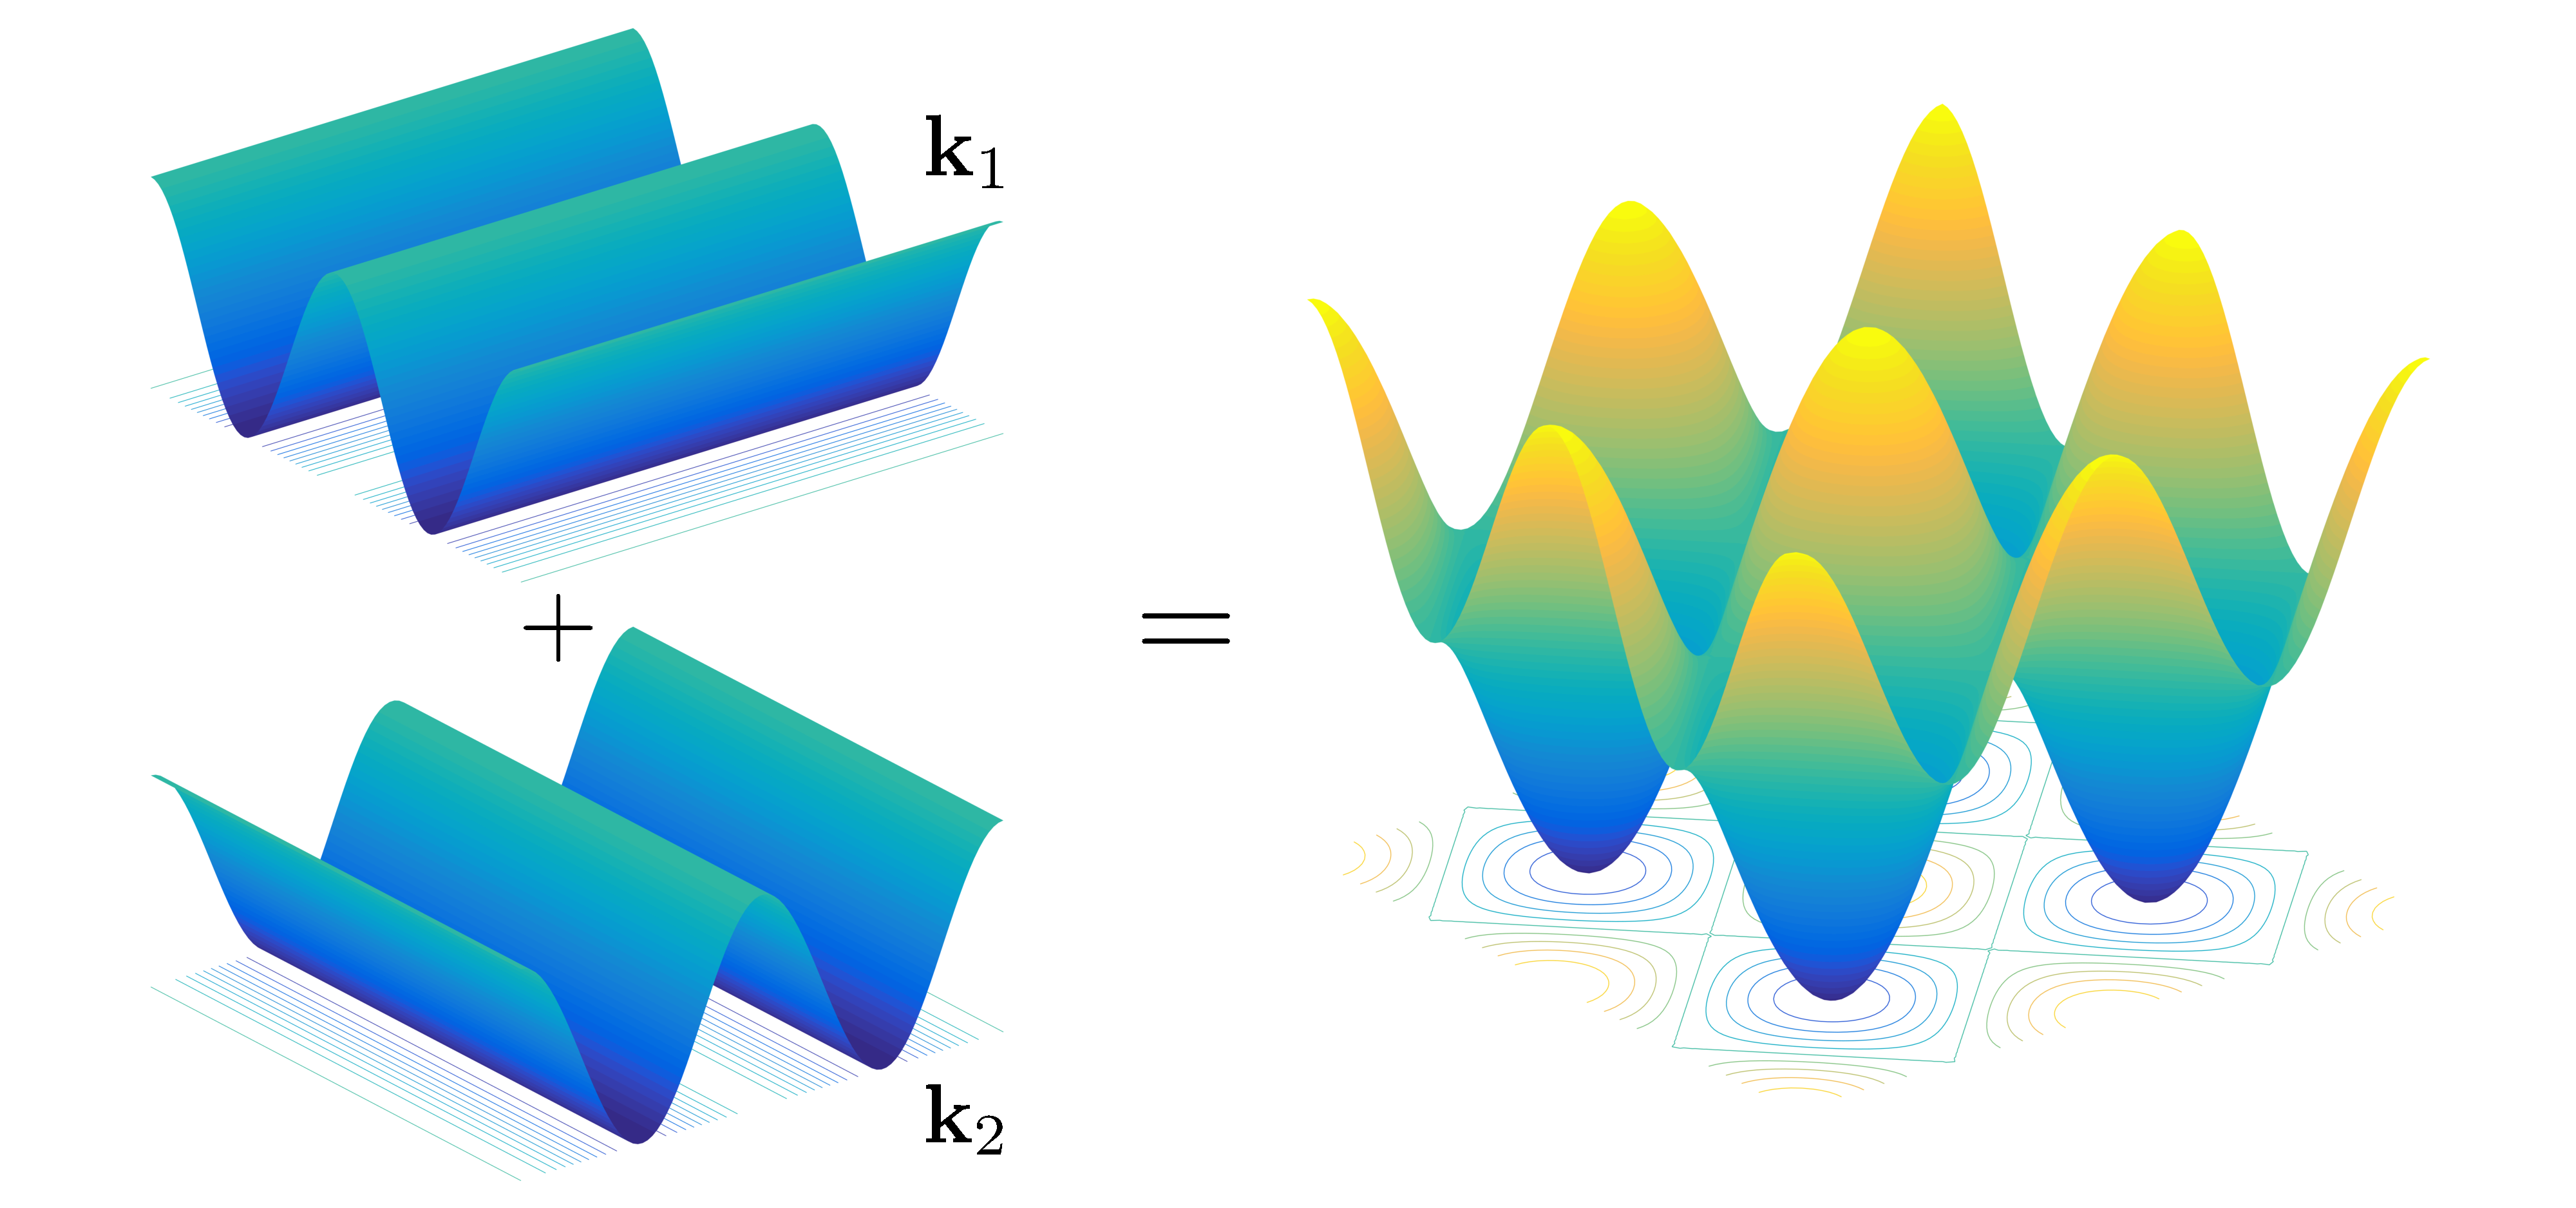
\includegraphics[width=0.75\textwidth]{./Images/ch4_vtx/VOPT/squarelatt}
    \caption{Square lattice generation using two orthogonal propagating laser fields, as defined by Eq.~\ref{eqn:sqlatt}.}\label{fig:cos2xy}
\end{figure}

By setting $H_1 = V_{\textrm{O}}$, the evolution of the condensate following the new additional potential can be controlled through use of $\alpha$. Given some time for evolution, the wavefunction phase will be modified and evolve due to the presence of the new potential. By assigning time-dependence to $\alpha$ one can effectively control the time of application of the optical potential. Experimentally, one can imagine this effect coming from the use of an optical shutter, and thus we can assume this is a realisable perturbation.

%%%%%%%%%%%%%%%%%%%%%%%%%%%%%%%%%%%%%%%%%%%%%%%%%%%%%%%%%%%%
\subsection{Phase imprinting defects}\label{sec:phase}
%%%%%%%%%%%%%%%%%%%%%%%%%%%%%%%%%%%%%%%%%%%%%%%%%%%%%%%%%%%%%%%%%%%%%%%%%%%%%%%%%%%%%%%%%%%%%%%%%%%%%%%%%%%%%%%%%%%%%%%%%%%%%%%%%%%%%%%%%%%%%

While previously I considered the use of a smoothly varying optical potential, one can also consider the case for a potential with a position-dependent intensity. Phase imprinting is a technique that applies a spatially inhomogeneous optical potential across a condensate in such a way that the phase is modified to a desired form. As a consequence the density distribution will adjust itself and in ground state condensates dark solitons \cite{BEC:Denschlag_science_2000}, as well as vortices \cite{Vtx:Dobrek_pra_1999} have been created this way. For the latter the signature is given by a phase singularity, around which the phase winds through $\pm 2\pi$, depending upon the direction of rotation. As discussed in Sec.~\ref{sec:}, this is the phase profile given for a quantum vortex, and by application of this pattern one can create such a topological defect in the wavefunction.

Where previously I added an optical potential to the Hamiltonian for a short time during the evolution, here I directly engineer the wavefunction phase.

%For the previously chosen kicking strengths and timestep, the limiting values of the phase change are $\approx 0.2 < \phi < \approx 0.94$. This is determined by writing the phase as
The previous method of applying the optical potential to the Hamiltonian in a time dependent manner and the phase imprinting method can be seen as performing the same operation. In one case, we modify the Hamiltonian for some time, $\tau$, and evolve the system under the new, and thereafter the old Hamiltonian, and in this scenario we apply a phase pattern directly to the wavefunction, wherein the physical realisation is observed using a strong optical pulse and a short application time. Comparison between the phase imprint and evolution can be seen by
\begin{equation}
    e^{i\phi} \mapsto \exp\left(-i\frac{V_{\textrm{O}}\tau}{\hbar}\right),
\end{equation}
where the phase of the wavefunction is given by the evolution in the presence of the new optical potential. Thus, for a much stronger phase change a longer lasting pulse, or a greater amplitude are two possible contenders. However, longer pulse durations are not ideal candidates in this system, as they may interfere with the overall dynamics of the wavefunction. With the use of direct phase imprinting we can realise arbitrary phase patterns on the condensate.



Previously the vortex lattice was unaffected by the imprint; here I attempt to destroy the vortex lattice by directly engineering the opposite phase winding profile atop a lattice vortex. This has the distinct advantage of locally erasing a vortex and disordering the lattice. I will now discuss this method.



The phase imprinting method can also be used to annihilate a vortex from the lattice by applying a phase profile of opposite winding, removing the phase singularity.  This will leave the condensate with a density depletion at the prior location of the phase singularity. Without the singularity this depletion will fill in and excite phonon modes in the condensate during time evolution. This method will form the basis for which the further discussions and analysis are performed on the vortex carrying condensate.






\section{Phase imprinting and manipulation}
Writing the wavefunction in the standard Madelung transform form, alongside a phase imprint term $\phi$ is given as
\begin{equation}
    \Psi(\mathbf{r},t) = |\Psi(\mathbf{r},t)|e^{\text{i}(\theta(\mathbf{r},t) + \phi(\mathbf{r}))}.
\end{equation}


%%% TO BE MOVED IN WITH PHASE ENGINEERING
Following \cite{BK:Pitaevskii_Stringari_2003} and taking the Madelung transform of the wavefunction given by Eq. \eqref{eqn:madelung}, the phase of the condensate may be specified as
\begin{equation}
\theta = \theta_c + \theta_i,
\end{equation}
where $\theta_c$ is the unperturbed condensate phase, and $\theta_i$ is the phase pattern to be imprinted. Thus, upon solving for the initial condensate phase, an additional phase pattern can be imprinted at any time by multiplying the wavefunction by the intended phase pattern. This is in line with the phase imprinting method, as previously introduced by Dobrek \textit{et al}. \cite{Vtx:Dobrek_pra_1999}.
%%% TO BE MOVED IN WITH PHASE ENGINEERING



\subsection{Gaussian phase}

\subsubsection{One dimensional}

\subsubsection{Two dimensional}



\section{Few vortex states}
As discussed in Section~\ref{sec:superfluid}, the discovery and manipulation of quantum vortices remains an active area of research.







Given that the energy of a vortex-carrying condensate scales as $E\propto l^2$, as $L_z \propto l$, any increase in the angular momentum causes a squared increase in the energy. Thus, for energetic favorability, the system prefers to maintain singly-charged vortices. To generate a vortex in the condensate costs energy,

Wi

\section{Quantum vortex dynamics}



\section{Vortex lattice states}
    \begin{equation}
        E(\Psi) = \int \Psi^{*} H_{\text GP} -\Omega L_z \Psi
    \end{equation}
